\documentclass[ a4paper,
                oneside,
                toc=bibliography,
                toc=listof
                ]{scrbook}

\usepackage[ngerman]{babel} % If the thesis is in English
%\usepackage[english, ngerman]{babel} % If the thesis is in German


% This class does the ISW styling for you (together with scrbook).
%
% It handles the following:
% - Proper input and font encoding (Just type, don't care about the LaTeX compiler you use or how to type German umlauts)
% - Fonts with ligatures and kerning (Tex Gyre fonts are used, part of every LaTeX installation, text is nice to read)
% - Bibliography styling for biblatex (declare your bibliography file and you are ready to go)
% - Provide command for title page (\makeISWtitle) and declaration of originality ( \declarationOfOriginality)
% - Loads packages "biblatex" and "graphics"
\usepackage[
    type=study, % master, bachelor, bachelorproject
]{iswthesis}

%Path to .bib-File(s) for BibLatex
\addbibresource{bibliography.bib}
% \addbibresource{someOtherBibFile}

\author{Lukas Schlotter}
\placeOfBirth{Stuttgart}
\major{Mechatronik}
\title{jbjhkbkj}
\titleTranslated{Wie man einen Hamster trainiert}
\matrnr{3668915}
\date{\today}
\supervisor{My supervisor, M.Sc.}
\professor{Prof. Dr.-Ing. Oliver Riedel}

\begin{document} 
    \frontmatter
    \makeISWtitle
    
    \cleardoublepage
	\setcounter{page}{1} % start at page (i) after title page
    %\declarationOfOriginality

    % Kurzfassung/Abstract
    
    \cleardoublepage
    \tableofcontents
    

    \mainmatter
    
    \chapter{Einleitung}
    Warum startet das hier mit ner 0?
    aTex allows you to manage citations within your document through the use of a separate bibtex file (filename.bib).
    
    
    \newpage
    
    Bibtex files follow a standard syntax that allow you to easily reference the citations included in that file through the use of a bibliography management package. There are multiple bibliography management packages that you can use to manage citations. \\
    This guide will demonstrate how to use biblatex which allows for the most customization.
    \section{Motivation}
    \begin{figure}[h]
    	\centering
    	
\includegraphics[width=1.0\linewidth]{./images/Test}
    	\caption{BPMN Prozess bei einem Taxiruf}
    	\label{fig:bpmn prozess}
    \end{figure}
    Dieses Bild zeigt blabla bla von dem Buch \cite{Tantau2013} und auch \cite{Kohm2013}
    
    \begin{table}[h!]
    	\centering
    	\begin{tabular}{||c c c c||} 
    		\hline
    		Col1 & Col2 & Col2 & Col3 \\ [0.5ex] 
    		\hline\hline
    		1 & 6 & 87837 & 787 \\ 
    		2 & 7 & 78 & 5415 \\
    		3 & 545 & 778 & 7507 \\
    		4 & 545 & 18744 & 7560 \\
    		5 & 88 & 788 & 6344 \\ [1ex] 
    		\hline
    	\end{tabular}
    	\caption{Table to test captions and labels.}
    	\label{table:1}
    \end{table}


	\chapter{Stand der Technik}
	
	\section{Feldbusse}
	Feldbusse: Elektrotechnik für Maschinenbauer ab S.485\\
	\\
	Feldbusse: Profibus, CAN, Sercos
	\\
	\\	
	Ethernet basierte Feldbusse: Profinet, Ethernet/IP, EtherCAT, Sercos III
	Ethernetbasierte Systeme sind bereit Feldbusse abzulösen
	
	\begin{figure}[h]
		\centering
		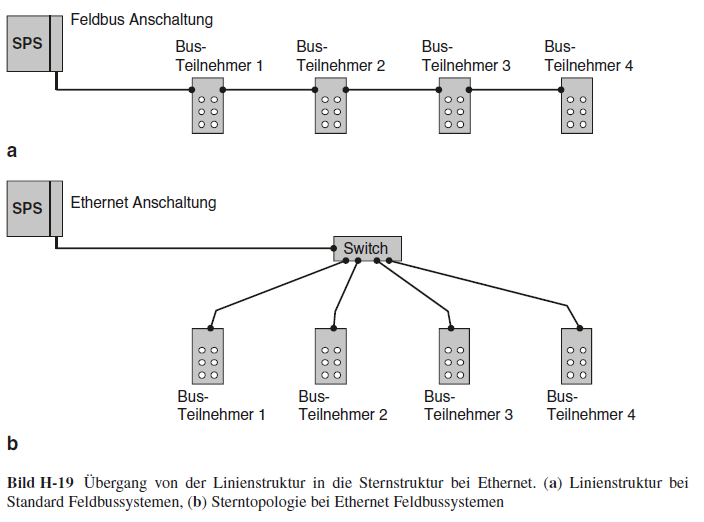
\includegraphics[width=1.0\linewidth]{./images/Feldbus vs Ethernet Anschaltung.png}
		\caption{Anschaltung Feldbus und Ethernet \cite{hering2012elektrotechnik}}
		\label{fig:Anschaltung Bus}
	\end{figure}
	
	\begin{figure}[h]
		\centering
		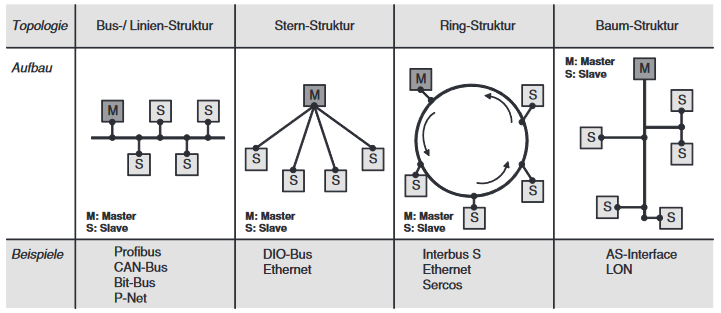
\includegraphics[width=1.0\linewidth]{./images/Topologien.png}
		\caption{Topologien}
		\label{fig:Topologien}
	\end{figure}
	Ethernet: deutlich mehr Daten als klassisch
	Multi-Master Bussen (z.B. CAN oder TCP/IP) vs. Mono-Master
	
	\section{TCP/IP}
   
   	MAC-Adresse eindeutig von Gerät. Für bessere Identifiuierung aber IP-Adresse
   	\begin{figure}[h]
   		\centering
   		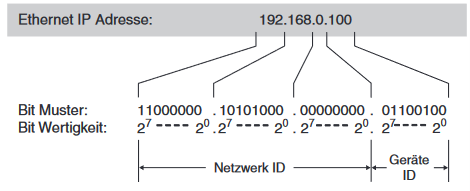
\includegraphics[width=0.70\linewidth]{./images/IP Adresse Aufbau.png}
   		\caption{Topologien}
   		\label{fig:Topologien}
   	\end{figure}
   \\
  Verschiedene Klassen an IP-Adressen. Meist Klasse C verwendet
  \\
  Weil Multi-Master-Bus braucht man CSMA/CD-Verfahren -> nicht echtzeitfähig. Lösung: Echtzeitprotokolle
  \\
  
  
   
   
    \backmatter
    \cleardoublepage
    \printbibliography

    \cleardoublepage
    \listoffigures
    \cleardoublepage
    \listoftables
    \cleardoublepage
    % Acronyms

    % Appendix, if needed:


\end{document}